\section{Motivation}

Representative datasets for Text-to-SQL include the WikiSQL\cite{zhong_seq2sql_2017} dataset and
the SPIDER\cite{yu_spider_2019} dataset, which contains more complex SQL queries.

The former case consists of Single Table - Multiple Question and the latter case Multiple Table - Multiple Question.
First, We will take a shallow look at older datasets and why they are no longer used in Text-to-SQL studies.
We will take a look at the difference between these datasets, which made a significant difference in the performance of Text-to-SQL systems.

The top language models and techniques utilized for the Text-To-SQL solution will be studied. We will jump into details of the architecture and backbond of these studies. We will evaluate the success of these researches and how they are different from each other.

After these models' performance review and hardware requirements, it is planned to develop a web application with minimum essentials for average users to access their database with their natural language questions without any SQL knowledge. This application will be open source via Github and accessible for enthusiasts to try this technology on their own.

% ? The state-of-the-art should show the reader a broad overview of techniques available and how they are related to one another in a hierarchical way like a mindmap. Describe the methods briefly and explain the weaknesses and strengths of the methods and how you want to use them to solve your problem.

\section{Background and Literature Review}

The text-to-SQL problem, or NL2SQL, is defined as the following: Given a Natural Language Query (NLQ) on a Relational Database (RDB), produce a SQL query equivalent to the NLQ. Several challenges include ambiguity, schema linking, vocabulary gaps, and user errors.

It has been a holy grail for the database community for over 30 years to translate user queries into SQL. During this section, we will provide a very brief overview of the earlier approaches, especially those that database communities have proposed.

% add image of mindmap here
\begin{figure}[htb]
    \centering
    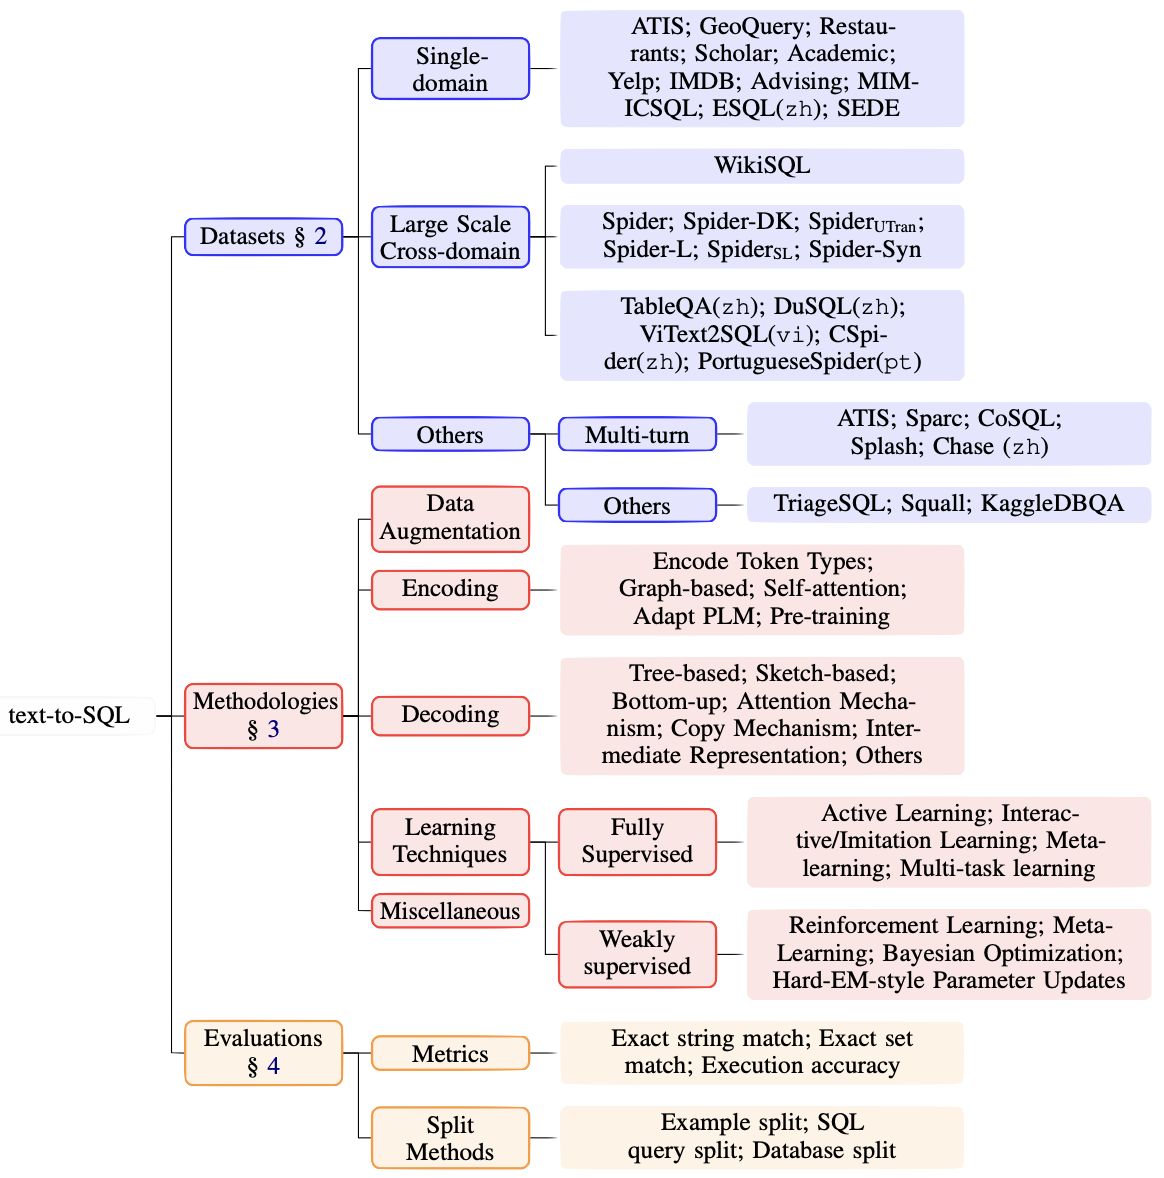
\includegraphics[width=0.6\textwidth]{pics/mindmap.png}
    \caption{Mindmap of the state-of-the-art}
    \label{fig:mindmap}
\end{figure}

\subsection{Early Approaches}

\subsection{Recent Approaches}
